\documentclass[12pt]{exam}		%Doc : https://mirrors.ircam.fr/pub/CTAN/macros/latex/contrib/exam/examdoc.pdf
\printanswers					%Comment this line to hide the answers 
\usepackage[utf8]{inputenc}
\usepackage[T1]{fontenc}
\usepackage[french]{babel}      %Originally for french document, change to english or relevant language

\usepackage{amsmath,amssymb}
\usepackage{multicol}
\usepackage[dvipsnames]{xcolor}
\usepackage[shortlabels]{enumitem}
\usepackage{tikz}
	\usetikzlibrary{fadings}
	\usetikzlibrary{calc}
	
\usepackage{tkz-tab}
\usepackage{pgfplots}

%Format Header and footer
\pagestyle{headandfoot}
\header{\footnotesize Class\\Id number}{\Large\textbf{Name}}
\headrule
\footrule
\setlength{\columnsep}{0.25cm}
%\setlength{\columnseprule}{1pt}
\footer{}{Page \thepage}{}
%\extrafootheight{-2cm}

% Change section command behaviour
\usepackage{titlesec}
\titleformat{\section}[frame]{\Huge\bfseries\filright}{}{2mm}{\centering Chemistry 123 :\ }

% Add a watermark if answers are shown
%\ifprintanswers
%\usepackage{draftwatermark}
%\SetWatermarkColor{red!30}
%\SetWatermarkScale{5}
%\SetWatermarkText{Solution}     %Watermark text
%\fi

%Format the name of each exercise
\qformat{\textbf{Exercice \thequestion~:}\hfill}
\extrawidth{1.5cm}

\begin{document}
\section{Exam 1B}

\noindent The 66 pts exam consists of 6 questions and students have the whole class period to complete the exam.
Answers must be written in the box provided or else no credit is provided. Use the empty
space provided to do your work. A periodic table is provided at the end. Fill in your name along with your
student ID number.
\\

\noindent\textbf{Problem 1: Empirical and Molecular Formulas} Caffeine, a
stimulant in coffee and tea, has a molar mass of 194.19 g/mol and a mass percentage
composition of $49.48\%$ C, $5.19\%$ H, $28.85\%$ N, and $16.48\%$ O. (8 pts)
\\
\begin{enumerate}[(a)]
\item Determine the empirical formula  %H2CO3
  \vspace{1in}
\item[]\tikz[baseline=1ex]\draw (0,0) rectangle (17cm,5ex);
\item What is the molecular formula of caffeine?  %NaHCO3
  \vspace{0.5in}
\item[]\tikz[baseline=1ex]\draw (0,0) rectangle (17cm,5ex);
\end{enumerate}

\noindent\textbf{Problem 2: Balancing Chemical Equations} Balance the following
chemical equations. (6 pts)
\\
\begin{enumerate}[(a)]
\item C$_3$H$_4$(g) + O$_2$(g) $\rightarrow$ CO$_2$(g) + H$_2$O(g)
  %
  \vspace{0.4in}
\item[]\tikz[baseline=1ex]\draw (0,0) rectangle (17cm,5ex);
\item H$_3$PO$_4$(aq) + Ca(OH)$_2$(aq) $\rightarrow$ Ca$_3$(PO$_4$)$_2$(s) + H$_2$O(l)
  % 2 H$_3$PO$_4$(aq) + 3 Ca(OH)$_2$(aq) $\rightarrow$ Ca$_3$(PO$_4$)$_2$(s) + 6 H$_2$O(l)
  \vspace{0.4in}
\item[]\tikz[baseline=1ex]\draw (0,0) rectangle (17cm,5ex);
\item Li(s) + H$_2$O(l) $\rightarrow$ LiOH(aq) + H$_2$(g)
  % 2 Li(s) + 2 H$_2$O(l) $\rightarrow$ 2 LiOH(aq) + H$_2$(g)
  \vspace{0.4in}
\item[]\tikz[baseline=1ex]\draw (0,0) rectangle (17cm,5ex);
\end{enumerate}

\newpage

\noindent\textbf{Problem 3: Significant Figures and Unit Conversion} Convert the following units and perform
the following calculations reporting the correct significant figures.(12 pts)
\\
\begin{enumerate}[(a)]
\item 8.58 cHz to $\mu$Hz %
  \vspace{0.45in}
\item[]\tikz[baseline=1ex]\draw (0,0) rectangle (17cm,5ex);
\item 8.16 dag/L to dg/mL %
  \vspace{0.45in}
\item[]\tikz[baseline=1ex]\draw (0,0) rectangle (17cm,5ex);
\item 1 m$^3$ to L (Hint: 1 mL = 1 cm$^3$) %
  \vspace{0.45in}
\item[]\tikz[baseline=1ex]\draw (0,0) rectangle (17cm,5ex);
\item 4.2 MJ to nJ %
  \vspace{0.45in}
\item[]\tikz[baseline=1ex]\draw (0,0) rectangle (17cm,5ex);
\item \begin{equation*}
  \frac{67.12 +52.013}{45.1} =
  \end{equation*}
\item[]\tikz[baseline=1ex]\draw (0,0) rectangle (17cm,5ex);\
\item \begin{equation*}
  5.192\times 10^2 - 1.024 \times 10 =
  \end{equation*}
\item[]\tikz[baseline=1ex]\draw (0,0) rectangle (17cm,5ex);
\end{enumerate}

\newpage

\noindent\textbf{Problem 4: Precipitation and REDOX Reactions} 
\\
\begin{enumerate}[(a)]
\item[] \textbf{Precipitation reaction}: Answer the following questions when mixing
  FeCl$_3$(aq) and KOH(aq). (8 pts)
  \begin{enumerate}[(i)]
  \item Write the balanced chemical equation when mixing FeCl$_3$(aq) and KOH(aq).
    Include the states.
  \item[]\tikz[baseline=1ex]\draw (0,0) rectangle (17cm,5ex);
  \item Write the complete ionic equation.
  \item[]\tikz[baseline=1ex]\draw (0,0) rectangle (17cm,5ex);
  \item What are the spectator ions?
  \item[]\tikz[baseline=1ex]\draw (0,0) rectangle (17cm,5ex);
  \item Write the net ionic equation.
  \item[]\tikz[baseline=1ex]\draw (0,0) rectangle (17cm,5ex);
  \end{enumerate}
\item[] \textbf{REDOX reaction}: Answer the following questions given the balanced
  chemical equation. (10 pts)
  \begin{center}
    Cu(s) + 2 AgNO$_3$(aq) $\rightarrow$ 2 Ag(s) + Cu(NO$_3$)$_2$(aq)
  \end{center}
  \begin{enumerate}[(i)]
  \item What are the oxidation states for each atom on the reactant side?
    \vspace{0.6in}
  \item[]\tikz[baseline=1ex]\draw (0,0) rectangle (17cm,5ex);
  \item What are the oxidationg states for each atom on the product side?
    \vspace{0.6in}
  \item[]\tikz[baseline=1ex]\draw (0,0) rectangle (17cm,5ex);
  \item What is the oxidizing agent?
  \item[]\tikz[baseline=1ex]\draw (0,0) rectangle (17cm,5ex);
  \item What is the reducing agent?
  \item[]\tikz[baseline=1ex]\draw (0,0) rectangle (17cm,5ex);
  \item From which atom to which atom, is the electron being transferred?
  \item[]\tikz[baseline=1ex]\draw (0,0) rectangle (17cm,5ex);
  \end{enumerate}
\end{enumerate}


\newpage

\noindent\textbf{Problem 5: Nomenclature} Provide either the chemical formula or
compound name for the following. (12 pts)
\\
\begin{enumerate}[(a)]
\item Vanadium(V) acetate %V(C2H3O2)5
\item[]\tikz[baseline=1ex]\draw (0,0) rectangle (17cm,5ex);
\item Sr(C$_2$H$_3$O$_2$)$_2$ %Strontium Acetate
\item[]\tikz[baseline=1ex]\draw (0,0) rectangle (17cm,5ex);
\item HClO$_3$ %Cloric acid
\item[]\tikz[baseline=1ex]\draw (0,0) rectangle (17cm,5ex);
\item (NH$_4$)$_2$SO$_4$ %Ammonium Sulfate
\item[]\tikz[baseline=1ex]\draw (0,0) rectangle (17cm,5ex);
\item Carbonic acid %H2CO3
\item[]\tikz[baseline=1ex]\draw (0,0) rectangle (17cm,5ex);
\item Sodium bicarbonate %NaHCO3
\item[]\tikz[baseline=1ex]\draw (0,0) rectangle (17cm,5ex);
\item AuP % Gold(III) phosphide
\item[]\tikz[baseline=1ex]\draw (0,0) rectangle (17cm,5ex);
\item SF$_6$ % Sulfur hexafluoride
\item[]\tikz[baseline=1ex]\draw (0,0) rectangle (17cm,5ex);
\item Potassium cyanide % KCN 
\item[]\tikz[baseline=1ex]\draw (0,0) rectangle (17cm,5ex);
\item Diphosphorus pentoxide % P$_2$O$_5$
\item[]\tikz[baseline=1ex]\draw (0,0) rectangle (17cm,5ex);
\item SO$_2$ % Sulfur dioxide
\item[]\tikz[baseline=1ex]\draw (0,0) rectangle (17cm,5ex);
\item Bi(NO$_3$)$_3$ % Bismuth(III) nitrite
\item[]\tikz[baseline=1ex]\draw (0,0) rectangle (17cm,5ex);
\end{enumerate}


\newpage

\noindent\textbf{Problem 6: Relative Atomic Mass and Molar Mass} Boron has only two naturally occurring
isotopes (Boron-10 and Boron-11). The mass of Boron-10 is 10.01294 amu and the mass of
Boron-11 is 11.00931 amu.(10 pts)
\\
\begin{enumerate}[(a)]
\item Calculate the relative abundance of each isotope. \textit{Hint:} There are two
  equations required.
  \vspace{1.75in}
\item[]\tikz[baseline=1ex]\draw (0,0) rectangle (17cm,5ex);
\item Taking the amu of boron from the periodic table, show conversion from amu to molar mass
  (g/mol). (1 amu = $1.661 \times 10^{-27}$ kg)
  \vspace{1in}
\item[]\tikz[baseline=1ex]\draw (0,0) rectangle (17cm,5ex);  
\end{enumerate}

\newpage

\appendix

\section{Apppendix 2 - Formulas and Constants}

\begin{align*}
  N_A & = 6.022 \times 10^{23} \text{particles/mol} \\
  \text{weighted average} & = A_1I_1 + A_2I_2 + \dots \\
  A_1 + A_2 + \dots & = 1
\end{align*}

\begin{center}
  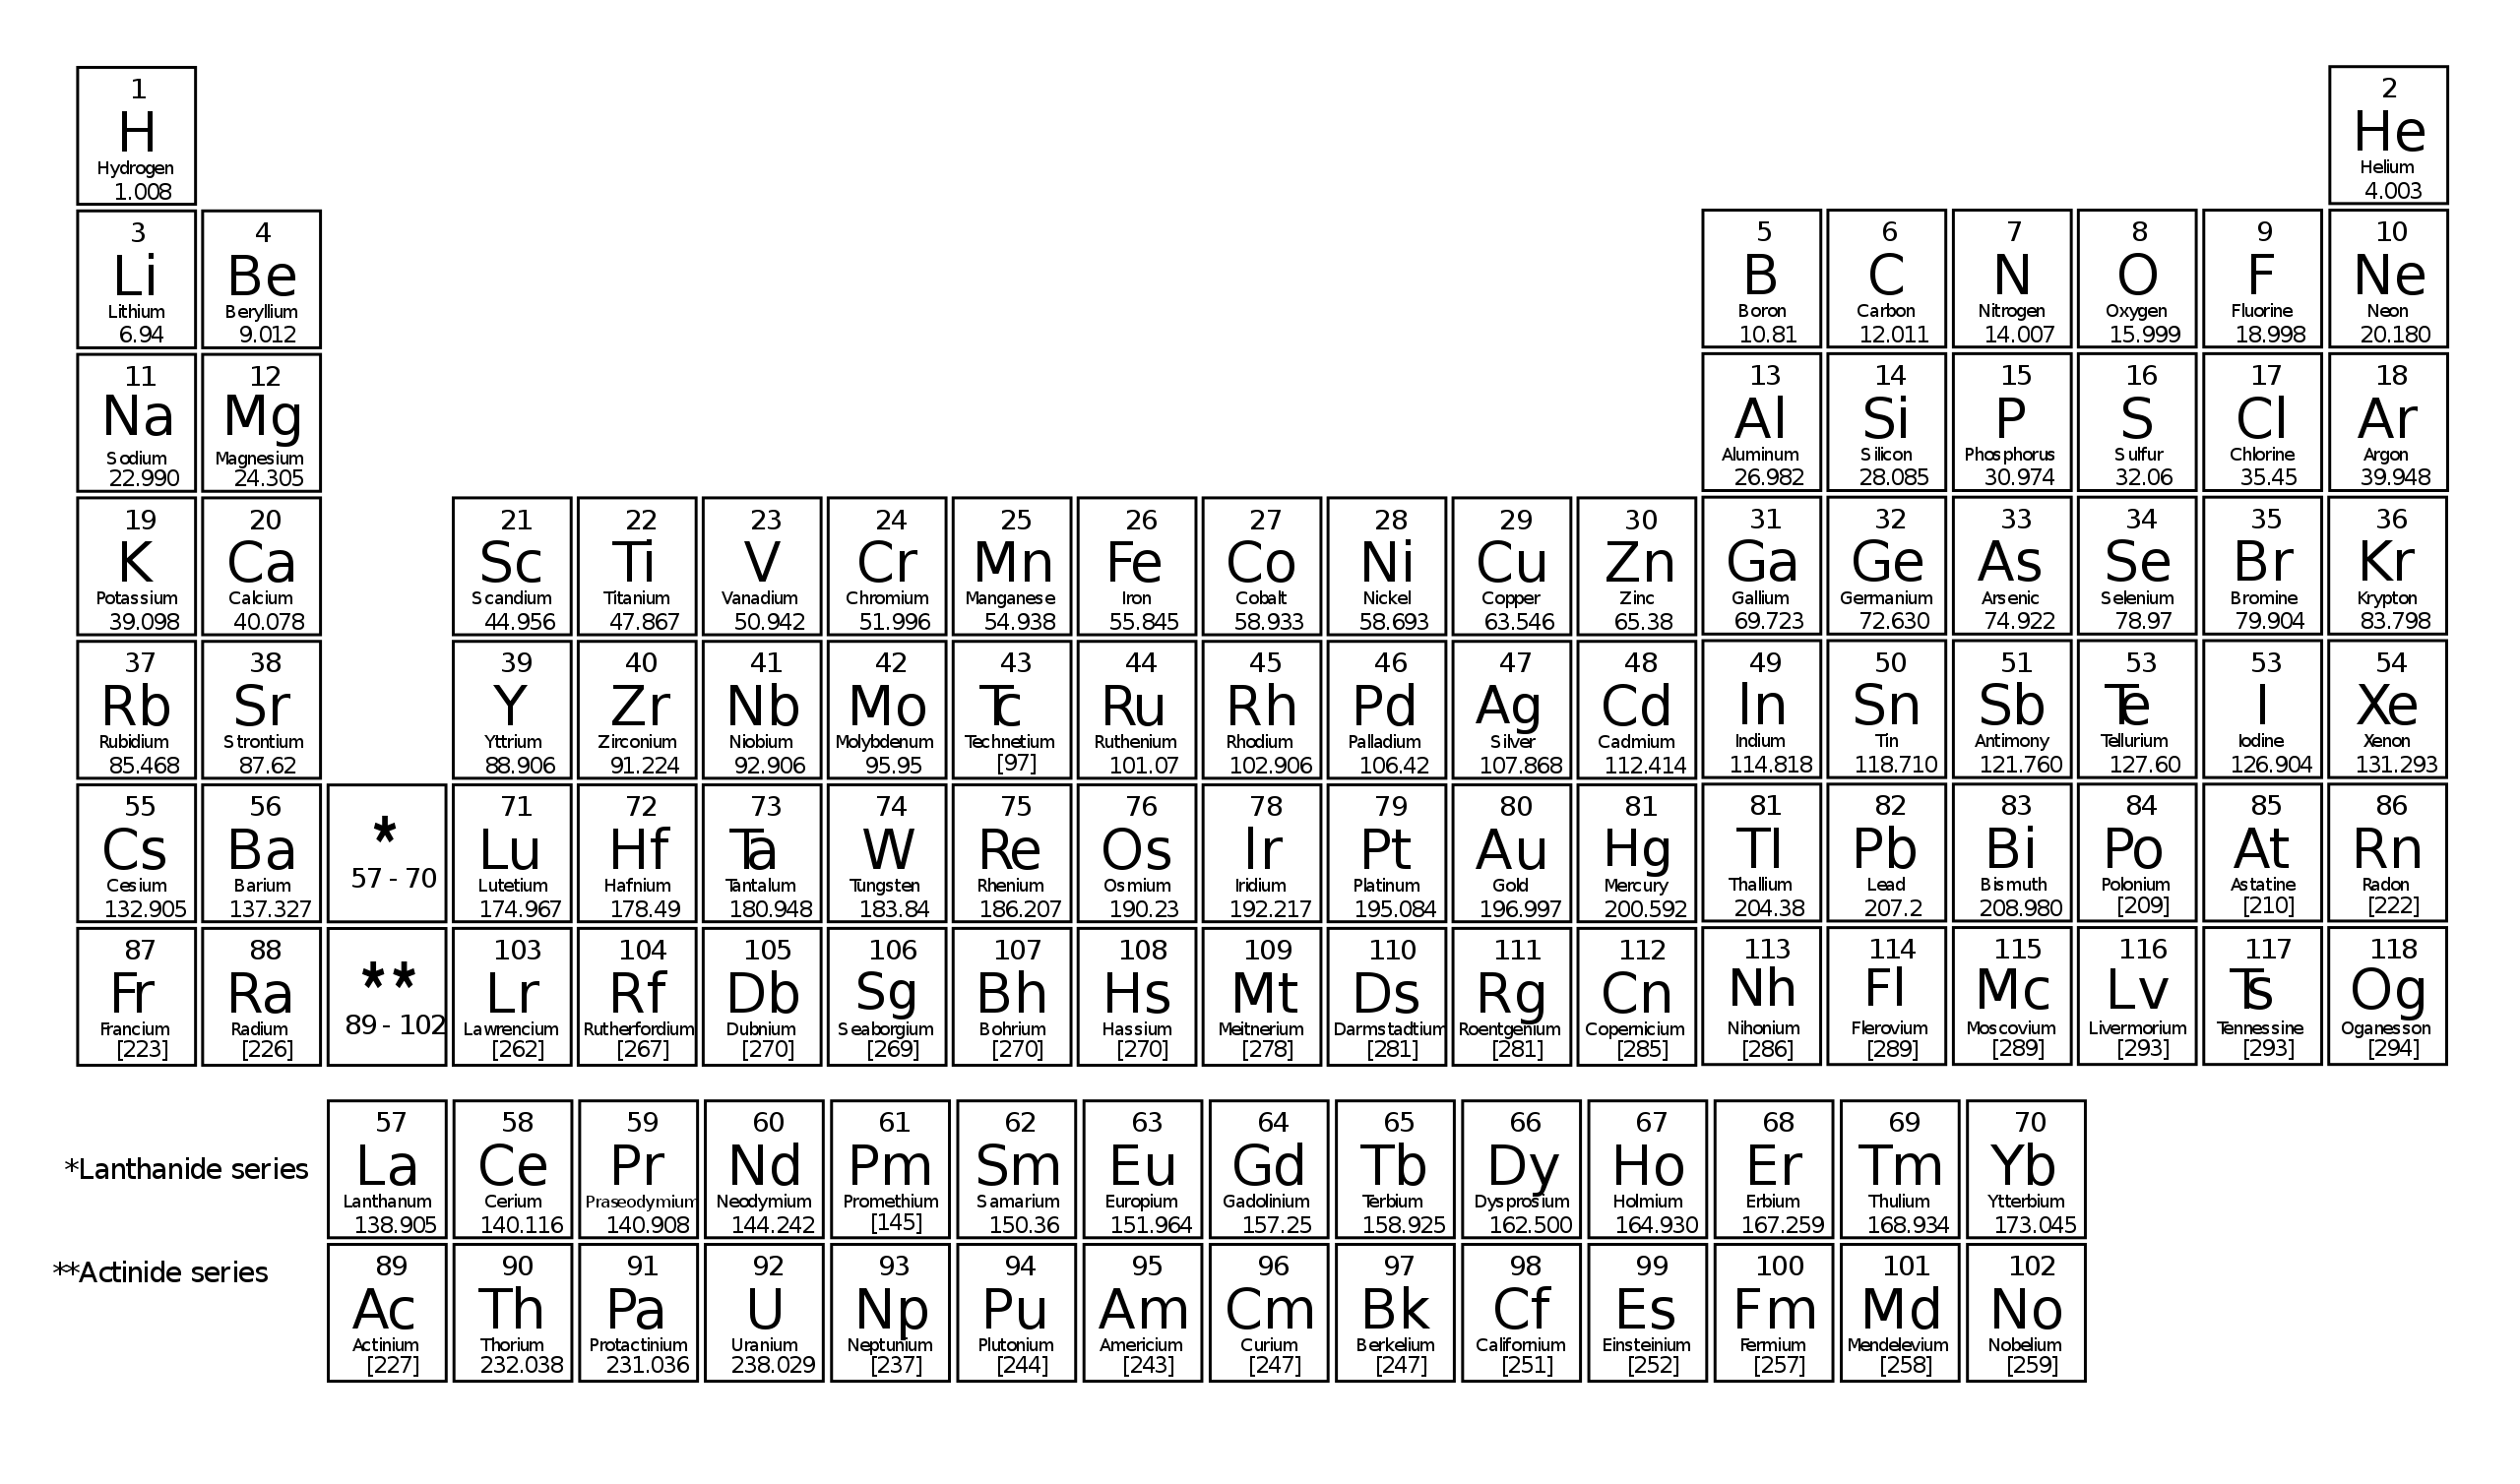
\includegraphics[scale=0.26,angle=90]{periodic_table}
\end{center}

\end{document}
